\documentclass[twocolumn]{article}
\usepackage{color}
\usepackage{amsmath}
\usepackage{amssymb}
\usepackage{xcolor}
\usepackage{tikz}
\usetikzlibrary{calc}
\usetikzlibrary{shapes.geometric}

\newcommand{\tenS}{\ensuremath{\mathcal{S}}}

\newcommand{\tenP}{\ensuremath{\mathcal{P}}}

\newcommand{\tenQ}{\ensuremath{\mathcal{Q}}}

\newcommand{\tenN}{\ensuremath{\mathcal{N}}}

\begin{document}

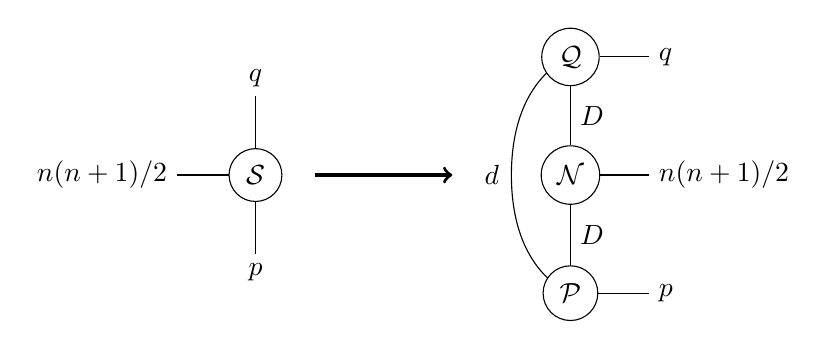
\begin{tikzpicture}
    \draw plot [smooth, tension=1.5] coordinates {(-0,-1.5) (-1.5/2,0) (-0,1.5)};
    \node[] at (-1.5/2- 0.25,0) {$d$};

    \node[draw, circle, fill=white] (S) at (-4,0) {$\tenS$};

    \node[draw, circle, fill=white] (P) at (0,-1.5) {$\tenP$};
    \node[draw, circle, fill=white] (Q) at (0,1.5) {$\tenQ$};
    \node[draw, circle, fill=white] (N) at (0,0) {$\tenN$};

    \draw[-] (P) -- (N) node[midway, right] {$D$};
    \draw[-] (N) -- (Q) node[midway, right] {$D$};


    \draw[-] (P) -- ++(1,0) node[right] {$p$};
    \draw[-] (Q) -- ++(1,0) node[right] {$q$};
    \draw[-] (N) -- ++(1,0) node[right] {$n(n+1)/2$};

    \draw[-] (S) -- ++(0,-1) node[below] {$p$};
    \draw[-] (S) -- ++(0,1) node[above] {$q$};
    \draw[-] (S) -- ++(-1,0) node[left] {$n(n+1)/2$};


    \draw[->, very thick] (-3.25,0) -- (-1.5,0);

\end{tikzpicture}

\end{document}